
\begin{figure}[H]
\centering
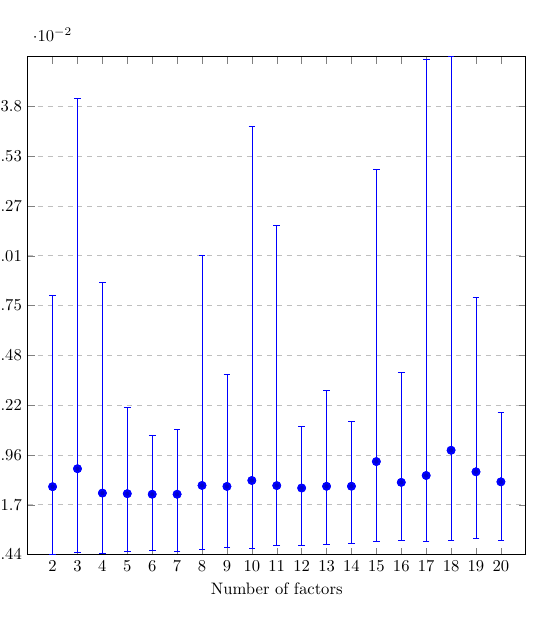
\begin{tikzpicture}[scale=0.6, trim axis left, trim axis right]
\begin{axis}[
    width=1\textwidth,
    height=1\textwidth,
    xlabel={Number of factors},
    ylabel={Time taken (s)},
    xmin=1.0, xmax=21.0,
    ymin=0.01435, ymax=0.040592,
    xticklabels={2, 3, 4, 5, 6, 7, 8, 9, 10, 11, 12, 13, 14, 15, 16, 17, 18, 19, 20},
    xtick={2, 3, 4, 5, 6, 7, 8, 9, 10, 11, 12, 13, 14, 15, 16, 17, 18, 19, 20},
    ytick={0.01435, 0.0169742, 0.0195984, 0.0222226, 0.0248468, 0.027471, 0.0300952, 0.0327194, 0.0353436, 0.0379678},
    ymajorgrids=true,
    grid style=dashed,
]

\addplot+[
    blue,
    very thick,
    forget plot,
    only marks
    ]
    plot[
    very thick,
    error bars/.cd,
    y dir=plus,
    y explicit
    ]
    table[x=x,y=y,y error expr=\thisrow{y-max}] {
    x    y    y-max
    11	0.01798465	0.01372335
10	0.0182553875	0.0186456125
13	0.0179480625	0.0050659375
12	0.01785825	0.00325575
15	0.019250975	0.015398025
14	0.0179509875	0.0034190125
17	0.0185172375	0.0219437625
16	0.0181557375	0.0058152625
19	0.018712425	0.009195575
18	0.019846275	0.020745725
20	0.0181835875	0.0036554125
3	0.0188752375	0.0195117625
2	0.0179269875	0.0100630125
5	0.017560425	0.004536575
4	0.0175914875	0.0111165125
7	0.0175302625	0.0033967375
6	0.0175300375	0.0030989625
9	0.0179422375	0.0059027625
8	0.017992975	0.012132025

    };

\addplot+[
    blue,
    very thick,
    forget plot,
    only marks
    ]
    plot[
    very thick,
    error bars/.cd,
    y dir=plus,
    y explicit
    ]
    table[x=x,y=y,y error expr=\thisrow{y-min}] {
    x    y    y-min
    11	0.01798465	-0.00315565
10	0.0182553875	-0.0035633875
13	0.0179480625	-0.0030550625
12	0.01785825	-0.00300725
15	0.019250975	-0.004193975
14	0.0179509875	-0.0029919875
17	0.0185172375	-0.0034482375
16	0.0181557375	-0.0030667375
19	0.018712425	-0.003511425
18	0.019846275	-0.004756275
20	0.0181835875	-0.0030775875
3	0.0188752375	-0.0043962375
2	0.0179269875	-0.0035769875
5	0.017560425	-0.003059425
4	0.0175914875	-0.0031724875
7	0.0175302625	-0.0030112625
6	0.0175300375	-0.0029590375
9	0.0179422375	-0.0032072375
8	0.017992975	-0.003359975

    };

\end{axis}
\end{tikzpicture}
\vspace{-0.3cm}
\caption{Large primes, close primes, modified algorithm}\label{fig:TrialDivisionLargecloseprimes(modified:True)factors}
\end{figure}
